\documentclass[pdftex,twocolumn,10pt,letterpaper]{extarticle}

%%% Set these variables appropriately
%%%
%% Note:  Authors is hardcoded below, this line only used for the PDF info
\newcommand{\AUTHORS}{Anuj Kalia and Dong Zhou}
\newcommand{\TITLE}{Understanding the PCIe Behavior of InfiniBand Network Cards}
\newcommand{\KEYWORDS}{Put your keywords here}
\newcommand{\CONFERENCE}{Somewhere}
\newcommand{\PAGENUMBERS}{yes}       % "yes" or "no"
\newcommand{\COLOR}{yes}
\newcommand{\showComments}{yes}
\newcommand{\comment}[1]{}
\newcommand{\onlyAbstract}{no}

%%%%%%%%%%%%%%%%%%%%%%%%%%%%%%%%%%%%%%%%%%%%%%%%%%%%%%%%%%%%%%%%%%%%%

%%%
%%%  Page Setup
%%%
\special{papersize=8.5in,11in}
\setlength{\pdfpagewidth}{8.5in}
\setlength{\pdfpageheight}{11in}

\usepackage{ifthen}
\ifthenelse{\equal{\PAGENUMBERS}{yes}}{%
\usepackage[nohead,
            left=0.75in,right=0.85in,top=0.75in,
            footskip=0.5in,bottom=1in,     % Room for page numbers
            columnsep=0.25in
            ]{geometry}
}{%
\usepackage[noheadfoot,left=0.75in,right=0.85in,top=0.75in,
            footskip=0.5in,bottom=1in,
            columnsep=0.25in
	    ]{geometry}
}

%%%
%%%  Captions
%%%
\usepackage[font=bf]{caption}
%%  Space between figure and caption (assuming caption
%%  is below figure)
%\usepackage[font=bf,aboveskip=0pt]{caption} % SPACE
%%  Space between caption and body text of document
%\addtolength{\textfloatsep}{-7pt} % SPACE

%%%
%%%  Section headings
%%%
\usepackage{titlesec}
%\titlespacing{\paragraph}{0pt}{*1}{*1}      % SPACE
%\usepackage[compact]{titlesec}              % SPACE
%\titleformat{\section}%                     % IEEE/ACM: caps + period
%  {\bf\large\uppercase}{\thesection.\quad}{0pt}{}

%%%
%%%  Lists
%%%
\usepackage{enumitem}
\setlist{itemsep=0pt,parsep=0pt}             % more compact lists

%%%
%%%  Header / Footer
%%%
\usepackage{fancyhdr}
\renewcommand{\headrulewidth}{0pt}

\ifthenelse{\equal{\PAGENUMBERS}{yes}}{%
  \pagestyle{plain}
}{%
  \pagestyle{empty}
}

%%%
%%%  Bibliography
%%%
\usepackage[numbers]{natbib}

%%%
%%%  Footnotes / Endnotes
%%%
\interfootnotelinepenalty=10000  % Split footnotes are annoying

% If you want endnodes, uncomment:
%\usepackage{endnotes}
%\usepackage{drafthead}
%\let\footnote=\endnote

%%%
%%%  Tables
%%%
\usepackage{booktabs}
\usepackage{color}
\usepackage{colortbl}
\usepackage{float}                           % Must appear before hyperref to
                                             % avoid weird PDF compile issues

%%%
%%%  Fonts
%%%
\usepackage{mathptmx}                        % Times/Times-like math symbols
\usepackage{courier}
\usepackage[scaled=0.92]{helvet}

%%%
%%%  PDF setup
%%%
\ifthenelse{\equal{\COLOR}{yes}}{%
  \usepackage[colorlinks]{hyperref}%         % for online version
}{%
  \usepackage[pdfborder={0 0 0}]{hyperref}%  % for paper (B&W) version
}
\usepackage{url}

\hypersetup{%
pdfauthor = {\AUTHORS},
pdftitle = {\TITLE},
pdfsubject = {\CONFERENCE},
pdfkeywords = {\KEYWORDS},
bookmarksopen = {true}
}

%%
%% Figure placeholder macros
%%

\definecolor{placeholderbg}{rgb}{0.85,0.85,0.85}
\newcommand{\placeholder}[1]{%
\fcolorbox{black}{placeholderbg}{\parbox[top][1.5in][c]{0.95\columnwidth}{#1}}}


%%%
%%%  Misc
%%%
\usepackage[pdftex]{graphicx}
\usepackage{soul}

%\setlength{\parindent}{0pt}
%\setlength{\parskip}{\baselineskip}

%\clubpenalty=10000  % Don't allow orphans
%\widowpenalty=10000 % Don't allow widows

%%%
%%%  To appear/appeared in text on title page
%%%
\usepackage[absolute]{textpos}
\newcommand{\ToAppear}{%
\begin{textblock*}{\textwidth}(0.95in,0.4in)
\begin{flushright}
    %\noindent{\fbox{\textsf{Under submission---please do not redistribute.}}}
    %  --OR--
    \noindent{\small To appear in \textit{Proceedings of the XYZ}\\
    \noindent{\small \textit{Conference (XYZ'08)}, City, State, Month 2008}}
    %  --OR--
    %\noindent{\small In \textit{Proceedings of the XYZ}\\
    %\noindent{\small \textit{Conference (XYZ'08)}, City, State, Month 2008}}
\end{flushright}
\end{textblock*}
}

%%%
%%%  Sample ACM Copyright Block
%%%
\newfloat{acmcr}{b}{acmcr}
\newcommand{\AcmCopyright}{%
\begin{acmcr}
\parbox[b]{20pc}{%
\footnotesize
Permission to make digital or hard copies of all or part of this work
for personal or classroom use is granted without fee provided that
copies are not made or distributed for profit or commercial advantage
and that copies bear this notice and the full citation on the first
page.  To copy otherwise, to republish, to post on servers or to
redistribute to lists, requires prior specific permission and/or a fee.

{\em Conference}, Month Date--Date, Year, Location\\
Copyright 200X ACM X-XXXXX-XX-X/XX/XX ...\$5.00}
\end{acmcr}}

%%%
%%%  Comments
%%%
\newcommand{\note}[2]{
    \ifthenelse{\equal{\showComments}{yes}}{\textcolor{#1}{#2}}{}
}

% Change these to your own initials as you like...
\newcommand{\dga}[1]{\note{blue}{Author1: #1}}
\newcommand{\mk}[1]{\note{red}{Author2: #1}}
\newcommand{\srini}[1]{\note{green}{Author3: #1}}

\date{}
\title{\textbf{\TITLE}}
\author{{\large {\AUTHORS}}\\}

% This needs to be the last thing before \begin{document}
%\usepackage{microtype}  % SPACE

%%%%%%%%%%%%%%%%%%%%  START DOCUMENT  %%%%%%%%%%%%%%%%%%%%%%%%
\begin{document}

\maketitle

%\AcmCopyright
%\ToAppear

\begin{abstract}
Understanding the low-level behavior of network interface cards (NICs) is an
important step towards building high-performance networked systems. In this
paper, we study one aspect of this behavior for InfiniBand network cards---the
interaction between the NIC and their PCI Express (PCIe) interface to
CPUs---using hardware counters.  While prior work presents a high-level picture
of this interaction~\cite{Kalia:sigcomm2014}, there is no existing emperical
measurement to the best of our knowledge.

We find two interesting behaviors. First, the PCIe behavior of non-batched and
batched RDMA operations is very different at the requester.  Second, we discover
evidence of a work request cache in the NICs, and suspect that the cache is
malfunctioning in the ConnectX-3 generation of InfiniBand NICs.

\end{abstract}

\ifthenelse{\equal{\onlyAbstract}{no}}{%
\section{Introduction}
\label{sec:intro}

Fast networks with Remote Direct Memory Access (RDMA) are becoming increasingly
popular.  Designing software systems to make the best use of these networks
is an interesting challenge because of the large design space. For example,
a key-value store atop RDMA can be designed with RDMA reads~\cite{Pilaf, FaRM},
RDMA writes~\cite{Kalia:sigcomm2014}, or a combination of both. Finding the
best design, as demonstrated by prior work~\cite{Kalia:sigcomm2014}, depends on
understanding the relative performance of different RDMA operations.

For small messages, the performance of RDMA operations is closely tied to their
behavior at the PCIe level. Avoiding unnecessary PCIe transactions can improve
performance by several factors, and is necessary to obtain the vendor's
advertized performance~\cite{Kalia:sigcomm2014}. Therefore, understanding the
\emph{exact} PCIe behavior of these operations is critical. While prior work
paints a rough picture of this behavior, which is also known through
word-of-mouth in the RDMA community, a measurement-based analysis of this
behavior is not available.

Part of the difficulty in understanding this behavior lies in the perceived
unavailability of PCIe measurement hardware. ASIC-based PCIe analysers are
expensive devices (over 10,000\$ for a PCIe 3.0 x16 analyser) and are not
widely available. However, we find that the PCIe counters found in Intel's
Xeon servers are sufficient for several measurements.

We make the following main contributions:
\begin{itemize}
\item We verify the PCIe behavior of RDMA read and write operations as
described in HERD~\cite{Kalia:sigcomm2014}.
\item We discover that the PCIe behavior of non-batched and batched RDMA
operations is very different, which has implications on their CPU usage and
peak throughput.
\item We discover evidence of a work request cache in Mellanox's RDMA adapters,
and suspect that it is malfunctioning in one adapter generation.
\item We document the working of PCIe counters in Intel's Xeon servers.
\end{itemize}

The rest of this paper is organized as follows. Section~\ref{sec:pcie} presents
a brief overview of PCIe express and InfiniBand/RDMA, and describes the
metrics reported by various PCIe counters. Section~\ref{sec:measurements}
presents the results from our PCIe measurements of different RDMA operations
on two generations of Mellanox's adapters. Section~\ref{sec:related} discusses
some related work. Section~\ref{sec:concl} discusses lines of future work and
concludes.

\section{PCIe and InfiniBand}
\label{sec:pcie}

This section discusses relevant details of PCI Express and InfiniBand, and
discusses what PCIe events are measured by Intel's PCIe counters on different
CPU generations.

\subsection{PCI Express}
PCIe is a serial point-to-point interconnect which is commonly used to connect
peripheral devices to a CPU. The bandwidth of a PCIe link is determined by two
factors: the link width and the PCIe generation. The link width speficies the
number of parallel lanes in the interconnect---the bandwidth of the link is
simply the per-lane bandwidth multiplied by the number of lanes. The PCIe
generation can be any number between 1 and 3, with PCIe 3.0 being the newest
generation at the time of writing. The transfer rate of a PCIe lane has
increased with each PCIe generation; Table~\ref{table:pcie} shows the transfer
rate of different PCIe generations and the bandwidth of a single lane of this
generation. As diffenent PCIe generations use different physical layer encodings
(8b/10b for PCIe 1.0 and 2.0, 128b/130b for PCIe 3.0), the relation between the
transfer rate and useful bandwidth of a PCIe lane depends on the generation. 

\begin{table}
\begin{center}
    \begin{tabular}{p{2.5cm} p{1.5cm} p{2.5cm}}
	\textbf{Generation} & \textbf{Bitrate} & \textbf{Lane bandwidth}\\
    \hline
	PCIe 1.0 & 2.5 GT/s & 250 MB/s \\
	PCIe 2.0 & 5 GT/s & 500 MB/s \\
	PCIe 3.0 & 8 GT/s & 984.6 MB/s \\
    \end{tabular}
\caption{Transfer rate and per-lane bandwidth of different PCIe generations}
\label{table:pcie}
\end{center}
\end{table}

\subsubsection{PCIe protocol}
PCIe is a layered protocol and consists of a physical layer, a link layer,
and a transport layer. The link layer uses credit-based flow control and
acknowledgments to provide reliable delivery to the transport layer.
Figure~\ref{fig:pcie-tlp} shows the structure of a PCIe 3.0 transaction layer
packet (PCIe TLP). In addition to the data payload, the packet includes physical
layer framing, a link layer sequence number (for reliability), a transport layer
header, and checksum at both the transport and link layer.

For the purposes of this paper, we assume that there are two types of PCIe
operations: memory read and memory write. The type of operation and the memory
address (in the peer's virtual memory) to read or write from is specified
in the transaction layer header. Therefore, the transaction layer
header can be either 12 or 16 bytes depending on whether 32-bit or 64-bit
addressing is used.  As almost all modern servers use 64-bit addressing, we
assume that the size of the transaction layer header is 16 bytes.

Note that the exact method of generating PCIe read and write transactions is
different for CPUs and NICs. The two common methods for generating these
transactions are Mapped Memory I/O (MMIO) and Direct Memory Access (DMA). MMIO
is used by the CPU to read or write the NIC's memory, whereas the NIC uses
DMA to read or write the CPU's memory. The efficiency of these two methods in
terms of CPU utilization (CPU utilization is reduced if a CPU-initiated MMIO
write can be replaced by a NIC-initiated DMA read) and PCIe bandwidth (MMIO
operations are restricted to a cacheline granularity) is different, which leads
to interesting optimizations and tradeoffs~\ref{sec:measurements}.

From Figure~\ref{fig:pcie-tlp}, it is clear that the minimum TLP overhead of
a PCIe packet is 30 bytes. This overhead is comparable to the common size of
data items used in networked services such as memcached~\cite{Nishtala:nsdi2013}
and RPCs~\cite{Flajslik:usenix2013}. Understanding and mitigating this overhead
can help in to designing RDMA-based communication protocols and networked
systems, as we will show in Section~\ref{sec:measurements}.

\begin{figure}
	\centering
	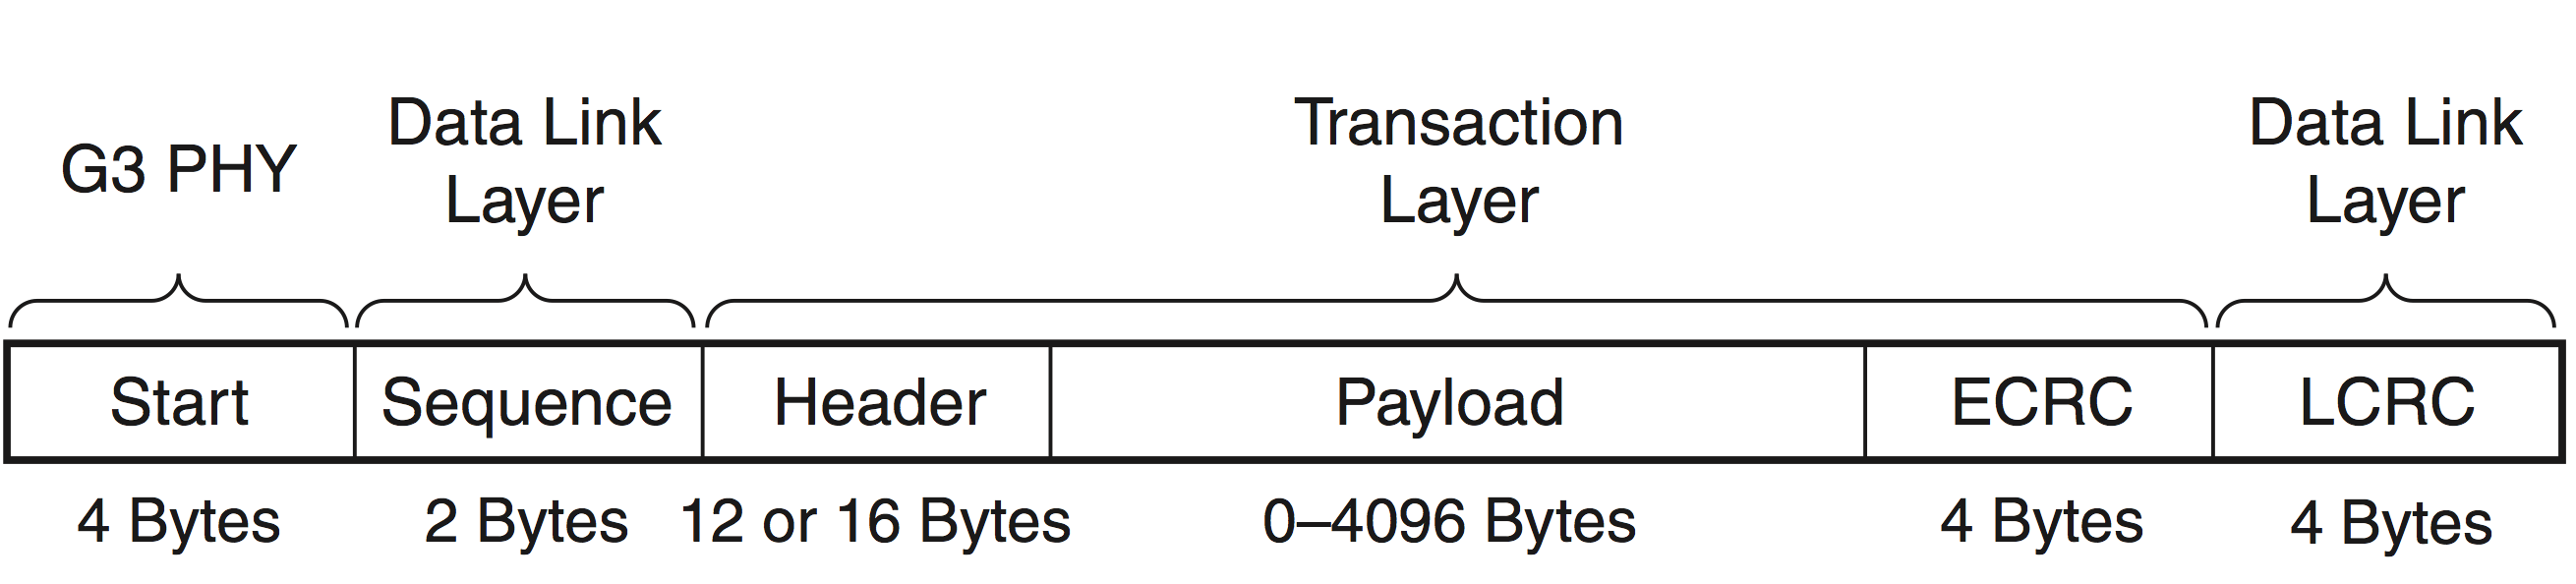
\includegraphics[width=.48\textwidth]{figures/pcie-tlp.png}
	\caption{\textbf{Structure of a PCIe TLP. The diagram was copied from~\cite{www-xilinx-pcie}}}
	\label{fig:pcie-tlp}
\end{figure}

\subsection{InfiniBand}
InfiniBand is standard for high-speed communication, commonly deployed between
two servers in a datacenters. InfiniBand focuses on low-latency and
high-bandwidth communication. The InfiniBand adapters used in this work have 56
Gbps of peak theoretical bandwidth per port, with $\sim$ 2 microseconds of
round-trip latency. All InfiniBand-compliant adapters must also provide RDMA.

\subsubsection{InfiniBand protocol and verbs}
Similar to PCIe, InfiniBand is a layered protocol. The header format of an
InfiniBand packet depends on several factors including the transport (connected
or datagram) and the type of RDMA operation (RDMA write or read or atomic). We
omit repeating all the header fields in this paper because they are irrelevant
from the PCIe point of view.

InfiniBand operations are also called ``verbs''. There are two main types of
verbs---memory verbs (RDMA READ and WRITE), which specify the remote memory
address to operate on, and messaging verbs (SENDs and RECVs), which behave
somewhat similarly to traditional UNIX sockets. The remote address to which the
payload of a SEND is written to is specified in a RECV that was previously
posted by the remote host.

\subsubsection{CPU-NIC interaction for RDMA}
InfiniBand communication uses queue pairs at the end hosts. To initiate an
InfiniBand operation, a user-level NIC driver at the requester host creates
a Work Queue Element (WQE) in host memory\footnote{We call the memory (cache
or DRAM) connected to a host CPU ``host memory'' and the memory (SRAM) of a NIC
``device memory''.}. The size of the WQE depends on several factors:
the type of InfiniBand operation, the InfiniBand transport, and whether or not
the data payload is ``inlined'' in the WQE. For example, excluding the optional
inlined data payload, an RDMA write WQE is 36 bytes in size. It consists of
16 byte control segment which contains the operation opcode and the queue pair
number of the remote peer's queue pair, a 16 byte ``remote address'' segment
which contains the address and permissions for the remote memory area to write
the data payload to, and a 4 byte data length field.


The WQE needs to be transferred from host memory to device memory over the
PCIe interconnect. There are 3 possible methods of doing this.

\begin{enumerate}
\item \textbf{Doorbell method}: The CPU writes to a memory-mapped register in
the NIC, alerting it of a new WQE. The NIC reads the WQE via a PCIe DMA read.
\item \textbf{BlueFlame method}: Using Mellanox's terminology, in the BlueFlame
method, the CPU writes the entire WQE to the NIC via MMIO.
\end{enumerate}

\section{Measurements}
\label{sec:measurements}
We conducted our measurements on the two hardware platforms described in
Table~\ref{tab:platforms}. As both platforms have SandyBridge CPUs, we were
unable to access PCIe counters for MMIO and partial cacheline DMA writes.
These counters are available on Haswell CPUs, and studying them is a part of
our future work.

\begin{table*}[h]
\begin{center}
    \begin{tabular}{p{2.5cm} p{6cm} p{10cm}}
	\textbf{Platform name} & \textbf{CPU} & \textbf{NIC}\\
    \hline
	Apt & Xeon E5-2450 (Sandy Bridge) & ConnectX-3 (single-port 56 Gb/s InfiniBand) via PCIe 3.0 x8 \\
	NetApp & Xeon E5-2670 (Sandy Bridge) & Connect-IB (dual-port 56 Gb/s InfiniBand) via PCIe 3.0 x16 \\
    \end{tabular}
\caption{Measurement platforms.}
\label{tab:platforms}
\end{center}
\end{table*}


%%%\section{Design}
\label{sec:design}

%%\section{Evaluation}
\label{sec:eval}

\begin{figure}
  \centerline{\placeholder{Descriptive figure text goes here.}}

\caption{A placeholder caption for a placeholder figure.}
\label{fig:placeholder}
\end{figure}

\section{Related Work}
\label{sec:related}

I like puppies~\cite{Andersen:nsdi2005}.

\section{Conclusion}
\label{sec:concl}

Therefore, a duck.


%\appendix
%\input{appendix_sources}

%\vspace{-0.1in}
%\section*{Acknowledgments}
% Comments for people we need to ack in the final version

%% Bibliography
\setlength{\bibsep}{2pt}
\small 
% \footnotesize % SPACE
\bibliography{ref}
\bibliographystyle{abbrvnat}
%\bibliographystyle{abbrvnat_noaddr} % SPACE
%\theendnotes % ENDNOTES
}{% !onlyAbstract
}

\end{document}

% Local Variables:
% TeX-command-default: "LaTeX PDF"
% End:

